% !TEX root = ../../main.tex

\section{Résultats numériques}
\label{sec:3:num}

Dans cette section on s'intéresse à des résultats numériques pour la résolution du modèle VHL par les méthodes présentées précédemment. Conformément à~\cite{Holderied:2020}, nous considérons la condition initiale suivante :
$$
  f_h(t=0,z,\vb{v}) = \frac{\rho_h}{(2\pi)^{3/2}\bar{v}_{\|}\bar{v}_\perp^2}\exp( - \frac{v_z^2}{2\bar{v}_{\|}^2} - \frac{\left( v_x^2 + v_y^2 \right)^2}{2\bar{v}_\perp^2} )
$$
avec $z\in[0,\frac{2\pi}{k}]$, $k=2$, $\bar{v}_{\|}=0.2$, $\bar{v}_\perp=0.6$, $\rho_h=0.2$ et $B_x(t=0,z)=\epsilon\sin(kz)$. Les autres inconnues du système $(j_{c,x},j_{c,y},B_y,E_x,E_y)$ sont initialisées à zéro. Le domaine en vitesse est restreint à $\vb{v}\in[-3.6,3.6]\times[-3.6,3.6]\times[-2.4,2.4]$ et on note $N_z$, $N_{v_x}$, $N_{v_y}$, $N_{v_z}$ le nombre de points de discrétisation dans chaque direction. Dans chacune des simulations, on s'intéresse à l'évolution temporelle des énergies suivantes :
\begin{description}
  \item[Énergie magnétique : ] \begin{equation}\label{eq:3:nrj:me}\mathcal{H}_B(t) = \frac{1}{2}\int \left( B_x^2(t,z) + B_y^2(t,z) \right)\dd{z}\end{equation}
  \item[Énergie électrique : ] \begin{equation}\label{eq:3:nrj:ee}\mathcal{H}_E(t) = \frac{1}{2}\int \left( E_x^2(t,z) + E_y^2(t,z) \right)\dd{z}\end{equation}
  \item[Énergie cinétique des particules froides : ] \begin{equation}\label{eq:3:nrj:ce}\mathcal{H}_c(t) = \frac{1}{2\Omega_{pe}^2}\int \left( j_{c,x}^2(t,z) + j_{c,y}^2(t,z) \right)\dd{z}\end{equation}
  \item[Énergie cinétique des particules chaudes :  ] \begin{equation}\label{eq:3:nrj:he}\mathcal{H}_h(t) = \frac{1}{2}\iint |\vb{v}|^2 f_h(t,z,\vb{v}) \dd{\vb{v}}\dd{z}\end{equation}
\end{description}
dont la somme, l'énergie totale, est préservée au cours du temps :
$$
  \dv{\mathcal{H}}{t} = \dv{\mathcal{H}_B+\mathcal{H}_E+\mathcal{H}_c+\mathcal{H}_h}{t} = 0.
$$
Les diagnostics que nous regarderons pour vérifier la validité des résultats sont les différentes énergies au cours du temps, en vérifiant le taux d'instabilité donné par les relations de dispersion, présentées dans~\cite{Holderied:2020}. La comparaison entre les méthodes de résolution se fera à partir de la préservation de l'énergie totale $\mathcal{H}$, et de l'erreur relative produite par chacune des méthodes, nous comparerons également les temps de calcul.

%%%%%%%%%%%%%%%%%%%%%%%%%%%%%%%%%%%%%%%%%%%%%%%%%%%%%%%%%%%%%%%%%%%%%

\FloatBarrier
\subsection{Comparaison des solveurs à pas de temps constant}
% -------------------------------------------------------------------

Dans un premier temps nous considérons la méthode de \emph{splitting} et de Lawson avec un pas de temps constant, comme présenté dans la section~\ref{sec:3:scheme}. Nous présentons trois méthodes de \emph{splitting}, à savoir les méthodes de Lie, Strang et de Suzuki. La méthode de Suzuki ne sera présente qu'à titre d'illustration mais celle-ci n'est pas très intéressante dans un contexte multidimensionel, en effet ses résultats sont très similaires à la méthode de Strang, mais son temps de calcul représente 5 fois celui de cette méthode d'ordre 2. Dès que l'hamiltonien se subdivise en de nombreuses parties (7 dans notre cas), le nombre d'étapes requises pour obtenir de l'ordre élevé augmente drastiquement (même si certaines stratégies peuvent être utilisées pour éviter cela, comme présentées dans~\cite{Casas:2017}). La méthode de Strang nécessite à elle seule 15 étapes, ce qui représente $5\times15=75$ étapes par itération, ce qui est trop important pour que la méthode soit compétitive. Nous présenterons également deux méthodes de Lawson, la méthode LRK(3,3) et LRK(4,4) induites respectivement par la méthode RK(3,3) de Shu-Osher et la méthode RK(4,4) dite classique. Contrairement aux méthodes de \emph{splitting}, les méthodes de Lawson ne sont pas trop impactées par la montée en ordre dans le sens où le nombre d'étages nécessaire correspond, \emph{à peu près}, à l'ordre de la méthode. De plus, il existe une souplesse intrinsèque aux méthodes de Lawson qui réside dans le choix de la partie linéaire. Ce choix permet, par exemple, de se soustraire de certaines conditions de stabilités, sous contrainte du calcul de l'exponentielle de cette partie, problème contourné dans la section~\ref{s3:approx}. De plus le filtrage possible du terme $\vb{v}\times\vb{B}$ est intéressant dans les méthodes de Lawson car il permet de relaxer la condition de stabilité de la méthode. Un filtrage similaire serait envisageable dans les méthodes de \emph{splitting}, avec comme coût l'ajout de sous-étapes supplémentaires dans l'étape $\mathcal{H}_{f_h}$, étape déjà la plus coûteuse numériquement.

L'utilisation de schémas explicites introduit une condition de stabilité dans la résolution des équations de Maxwell, dans les deux approches (méthode de \emph{splitting} et de Lawson), présentée dans~\cite{Kormann:2021}. Il est également possible de se concentrer uniquement sur les inconnues $(B_x,B_y,E_x,E_y)$ pour déduire une condition de stabilité, comme vu dans la sous-section~\ref{ssec:3:cflMaxwell}. Le tableau~\ref{tab:CFL_maxwell} résume les différentes conditions de stabilité. Pour les méthodes de Lawson une condition de CFL supplémentaire provient de la discrétisation en vitesse, mais on remarque numériquement que cette dernière est moins contraignante que la condition provenant des équations de Maxwell. Nous verrons dans la section~\ref{s3:approx} comment s'affranchir de cette condition en intégrant les équations de Maxwell dans la partie linéaire de la méthode de Lawson.

\begin{table}[h]
  \centering
  \begin{tabular}{c|c}
    méthode         & condition de CFL          \\
    \hline
    Lie             & $(\sqrt{2}/\pi) \Delta z$ \\ 
    Strang          & $(2/\pi)\Delta z$         \\
    Lawson-RK(3, 3) & $(\sqrt{3}/\pi)\Delta z$  \\ 
    Lawson-RK(4, 4) & $(2\sqrt{2}/\pi) \Delta z$  
  \end{tabular}
  \caption{Condition de stabilité provenant des équations de Maxwell en utilisant différents intégrateurs.} 
  \label{tab:CFL_maxwell}
\end{table}

Nous traçons, sur la figure~\ref{fig:energies4d} l'évolution des énergies électrique, magnétique et l'énergie cinétique provenant des particules froides, définies précédemment, en échelle semi-log, pour différentes méthodes de \emph{splitting} (méthode de Lie, de Strang, et de Suzuki), et différentes méthodes de Lawson (LRK(3,3) et LRK(4,4), l'adjectif \emph{filtred} fait référence au filtrage mis en place dans la section~\ref{ssec:3:filtrage}). On choisit le maillage $27\times32\times32\times41$ et $\Delta t=0.05$ (ce qui assure la stabilité de toutes les méthodes présentées). On considère une faible perturbation $\epsilon = 10^{-5}$, pour assurer une longue phase linéaire (jusqu'au temps $t\approx 100$) tandis que la phase non-linéaire se développe jusqu'au temps final $t=200$. Dans la partie linéaire, il est possible de comparer les résultats numériques avec les solutions des relations de dispersion présentées dans~\cite{Holderied:2020}. Comme attendu, les trois énergies suivent une croissance exponentielle, avec le taux prédit par la théorie linéaire, ce qui se traduit par des transferts d'énergie des particules rapides (chaudes) vers l'énergie électro-magnétique et aux particules froides. Après la phase linéaire, les champs saturent en amplitude, ce qui marque l'effet des termes non-linéaires, la théorie linéaire n'est plus valide. On remarque que les deux classes de méthodes capturent efficacement les différents phénomènes en jeu dans la phase linéaire, avec une très bonne corrélation avec les taux d'instabilités calculés à l'aide de la théorie linéaire. De plus les différentes méthodes saturent à des niveaux d'énergie très similaires.

La figure~\ref{fig:energy_tot4d} représente l'erreur relative sur l'énergie totale, et permet d'étudier la conservation de celle-ci par les différentes méthodes. Bien que le maillage en espace soit très grossier ($\Delta z = \frac{2\pi}{27} \approx 0.23$) l'énergie totale est plutôt bien préservée : aux alentours de $8\%$ pour les deux méthodes de Lawson présentées, et autour de $5\%$ d'erreur pour les méthodes de Lie et de Strang. La méthode de Suzuki produit bien plus d'erreur (autour de $12\%$) très certainement à cause des multiples transformées de Fourier selon l'axe $z$ effectuées avec peu de points de discrétisation. Comme attendu, et observé dans le cas $1dx-1dv$, les méthodes basées sur un \emph{splitting} hamiltonien ont une bonne préservation de l'énergie totale, mais les qualités de leurs résultats, surtout observable avec la méthode de Suzuki, suggère la nécessité de raffiner le maillage. Il est à souligner que le coût numérique de la méthode de Strang, est environ deux fois plus important que celui de la méthode LRK(3,3).

\begin{figure}[h]
  \centering
  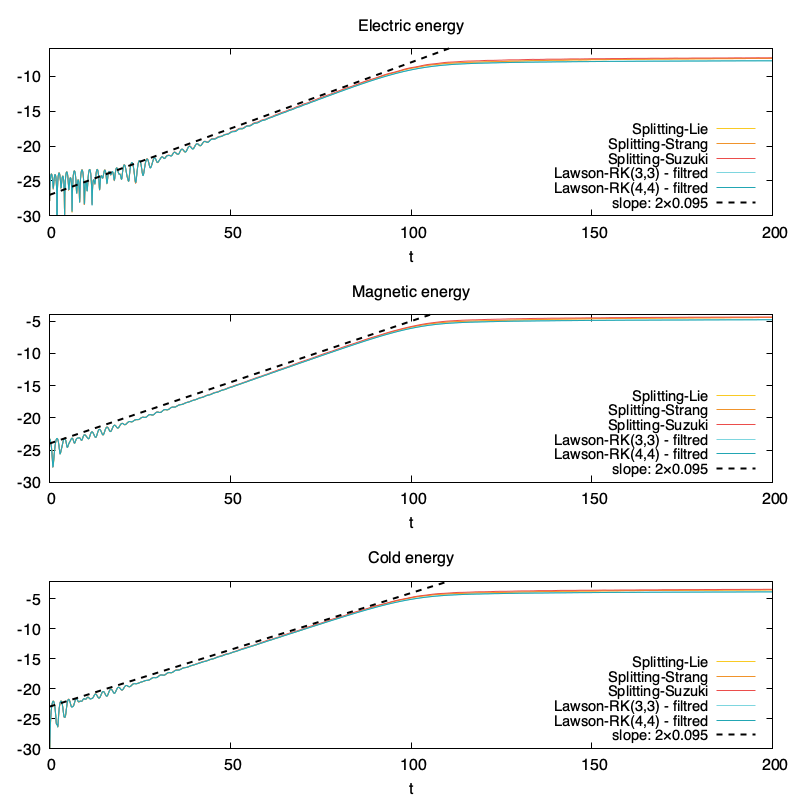
\includegraphics[width=0.9\textwidth]{\localPath/figures/energy_a_vmhl.png}
  \caption{Évolution de l'énergie électrique, magnétique et l'énergie cinétique des particules froides définies dans les équations~\ref{eq:3:nrj:me}-\ref{eq:3:nrj:ce}, en échelle semi-$\log$, pour les méthodes de \emph{splitting} de Lie, Strang et Suzuki, et pour les méthodes de Lawson LRK(3,3) et LRK(4,4). $\Delta t = 0.05, N_x=27, N_{v_x}=32, N_{v_y}=32, N_{v_z}=41$.}
  \label{fig:energies4d}
\end{figure}

\begin{figure}[h]
  \centering
  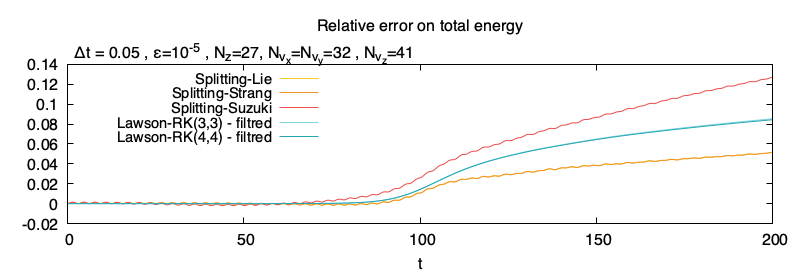
\includegraphics[width=0.9\textwidth]{\localPath/figures/H_a_vmhl.png}
  \caption{Évolution de l'erreur relative sur l'énergie totale, pour les méthodes de \emph{splitting} de Lie, Strang et Suzuki, et pour les méthodes de Lawson LRK(3,3) et LRK(4,4). $\Delta t = 0.05, N_x=27, N_{v_x}=32, N_{v_y}=32, N_{v_z}=41$.}
  \label{fig:energy_tot4d}
\end{figure}

On peut étudier l'importance du filtrage du terme $\vb{v}\times\vb{B}$ avec la figure~\ref{fig:compar_ee4d}, où l'on trace l'évolution de l'énergie électrique pour la méthode de Lawson LRK(3,3) avec ou sans le filtrage (voir l'algorithme~\ref{alg:modif} pour la différence algorithmique entre les deux méthodes) pour deux maillages différents de l'espace des phases ($15\times20\times20\times41$ à gauche et $15\times32\times32\times41$ à droite) avec un pas de temps $\Delta t = 0.1$. On peut observer l'impact sur les résultats du raffinement dans la direction $v_\perp$ sur la méthode non-filtrée, alors que sur la méthode filtrée on obtient un taux d'instabilité satisfaisant avec le maillage le plus grossier.

\begin{figure}[h]
  \centering
  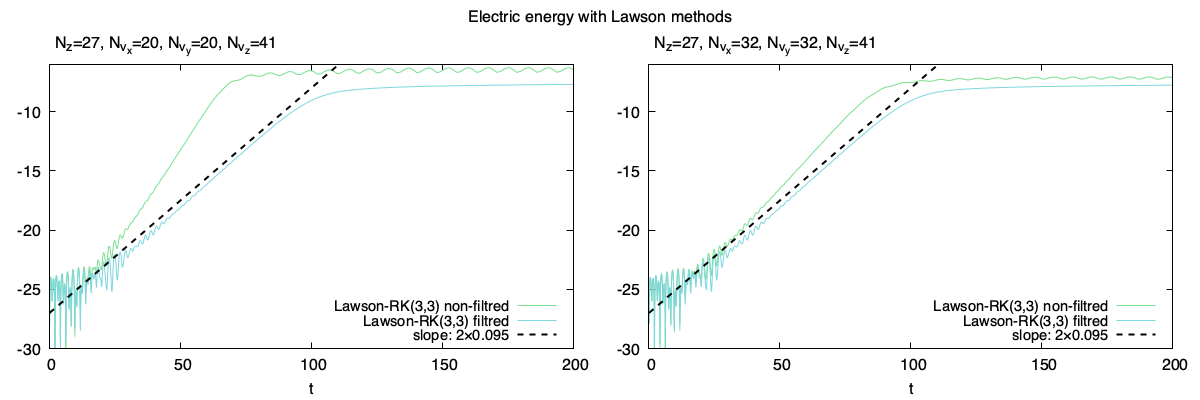
\includegraphics[width=0.9\textwidth]{\localPath/figures/ee_filtrage_vmhl.png}
  \caption{Évolution de l'énergie électrique pour les versions filtrées et non-filtrées de la méthode LRK(3,3) avec des maillages en vitesse différents. À gauche : $\Delta t = 0.05, N_x=27, N_{v_x}=20, N_{v_y}=20, N_{v_z}=41$. À droite : $\Delta t = 0.05, N_x=27, N_{v_x}=32, N_{v_y}=32, N_{v_z}=41$.}
  \label{fig:compar_ee4d}
\end{figure}


%%%%%%%%%%%%%%%%%%%%%%%%%%%%%%%%%%%%%%%%%%%%%%%%%%%%%%%%%%%%%%%%%%%%%

\FloatBarrier
\subsection{Étude à pas de temps adaptatif}
% -------------------------------------------------------------------
\label{ssec:3:dtn}

Le dernier test que nous souhaitons effectuer avec ces méthodes de résolution, est de considérer la méthode de Lawson à pas de temps adaptatif induite par le schéma DP4(3), comme dans la section \ref{ssec:dtadapt}. Pour que l'approche à pas de temps adaptatif soit intéressante dans notre cas il faut que :
\begin{enumerate}[label=(\roman*)]
  \item Les champs électromagnétiques soient suffisamment faibles dans la phase linéaire pour pouvoir prendre des grands pas de temps,\label{list:i}
  \item La condition de stabilité provenant des équations de Maxwell ne soit pas trop restrictive,\label{list:ii}
  \item Dans la phase non-linéaire, l'estimateur d'erreur nous assure la stabilité.\label{list:iii}
\end{enumerate}
En pratique, à cause de la discrétisation en espace la condition~\ref{list:ii} n'est pas satisfaite. Pour la suite nous considérons les paramètres numériques suivant : $N_z=27$, $N_{v_x}=32$, $N_{v_y}=32$, $N_{v_z}=41$, $tol=6\times10^{-5}$ et le pas de temps calculé par :
$$
  \Delta t_0 = \frac{C}{2}\Delta z,\quad \Delta t_{n+1} = \min\left( \max\left( \sqrt[p]{\frac{tol}{L_{[p]}^{n+1}}}\Delta t_n ,\frac{C}{2}\Delta z \right) , 3C\Delta z \right), n\geq 0
$$
où $L_{[p]}^{n+1}$ est l'erreur locale calculée par~\ref{eq:Lerror}, et $C$ est donné par le tableau~\ref{tab:CFL_maxwell}. La figure~\ref{fig:energieselecdp43} montre l'énergie électrique en échelle semi-log. Comme pour les méthodes présentées dans la section~\ref{ssec:2:dtn} les résultats sur les énergies sont très similaires, on capture le bon taux d'instabilité. On regarde sur la figure~\ref{fig:dtanderrordp43} deux diagnostics sur la méthode LDP4(3). Tout d'abord l'évolution de la taille des pas de temps au cours du temps (figure du haut). La simulation avec LDP4(3) est initialisée avec un pas de temps $\Delta t_0=0.05\approx\frac{1}{2}\frac{2\sqrt{2}}{N_z}$, les 3 itérations suivantes sont effectuées avec le pas de temps $\Delta t_n=3\frac{2\sqrt{2}}{N_z}$ qui est la borne supérieure que peut prendre le pas de temps $\Delta t_n$ (pour minimiser l'erreur générée en début de simulation, les champs électromagnétiques étant très faibles, l'estimateur d'erreur $L_{[p]}^{n+1}$ permet de prendre des pas de temps supérieurs à $1$) ; les autres itérations sont effectuées avec un pas de temps très proche de la condition de stabilité provenant des équations de Maxwell. Dans la phase linéaire, jusqu'au temps $t\approx 100$, la condition~\ref{list:ii} n'est pas satisfaite, la résolution des équations de Maxwell impose une condition CFL forte. Dans la phase non-linéaire, du temps $t\approx100$ jusqu'au temps final $t=200$, la condition de stabilité induite par le transport dans les directions $(v_x,v_y,v_z)$ n'est pas trop contraignante, ce qui permet de satisfaire la condition~\ref{list:iii} avec une contrainte pas trop forte. On remarque tout de même que la méthode LDP4(3) permet de prendre des pas de temps légèrement supérieurs à cette condition de stabilité, en effet $16\%$ des itérations réussies ont un pas de temps $\Delta t_n$ supérieur à la condition de stabilité $\frac{2\sqrt{2}}{N_z}$. La deuxième partie de la figure~\ref{fig:dtanderrordp43}, celle-du bas, présente l'erreur locale au cours du temps, sont tracées également, par des carrés, les itérations rejetées. Contrairement au cas $1dx-1dv$, où le surcoût engendré par les itérations rejetées était négligeable, ici, seulement $71\%$ des itérations sont acceptées par le critère d'erreur.

\begin{figure}[h]
  \centering
  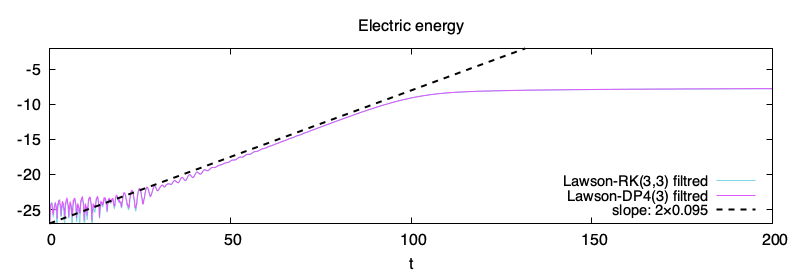
\includegraphics[width=0.77\textwidth]{\localPath/figures/energy_dp43_vmhl.png}
  \caption{Évolution de l'énergie électrique définie dans~\eqref{eq:3:nrj:ee}, en échelle semi-$\log$ pour les méthodes LRK(3,3) ($\Delta t = 0.05$) et LDP4(3). $N_x=27, N_{v_x}=32, N_{v_y}=32, N_{v_z}=41$.}
  \label{fig:energieselecdp43}
\end{figure}

\begin{figure}[h]
  \centering
  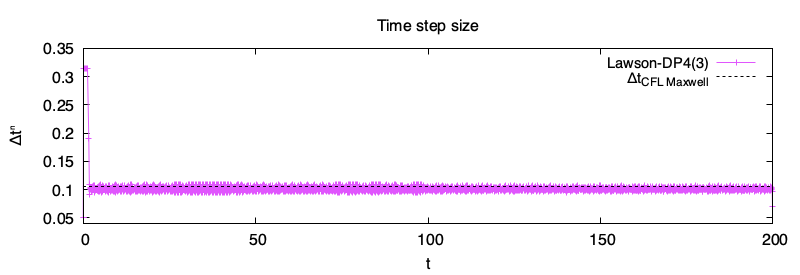
\includegraphics[width=0.77\textwidth]{\localPath/figures/dt_size_vmhl.png}
  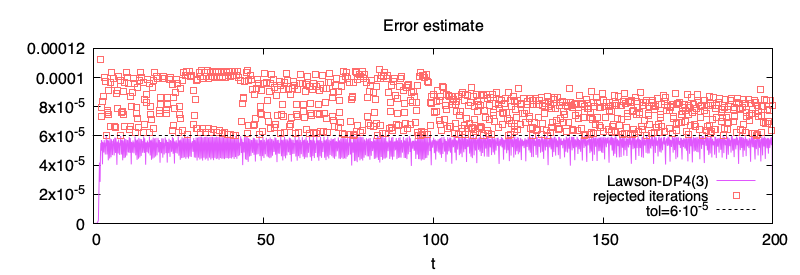
\includegraphics[width=0.77\textwidth]{\localPath/figures/L_vmhl.png}
  \caption{Évolution au cours du temps de la taille du pas du temps (haut) et de l'erreur locale (bas) pour la méthode de Lawson LDP4(3). $N_x=27, N_{v_x}=32, N_{v_y}=32, N_{v_z}=41$.}
  \label{fig:dtanderrordp43}
\end{figure}

